\documentclass[12pt, a4paper, hidelinks]{article}

% Packages:
\usepackage{graphicx}                   % For figure includes
\usepackage[T1]{fontenc}                % For mixing up \textsc{} with \textbf{}
\usepackage[utf8]{inputenc}             % For scandinavian input characters(æøå)
\usepackage{amsfonts, amsmath, amssymb} % For common mathsymbols and fonts
\usepackage[english]{babel}              % For danish titles
\usepackage{hyperref}                   % For making links and refrences
\usepackage{url}                        % Just because {~_^}
\usepackage{array}                      % ...
\usepackage[usenames, dvipsnames, svgnames, table]{xcolor}
\usepackage{tabularx, colortbl}
\usepackage{verbatim} % For entering code snippets.
\usepackage{fancyvrb} % A "fancy" verbatim (for pseudo code).
\usepackage{listings} % For boxed codesnippets, and file includes. (begin)
\usepackage{lipsum}   % For generating dummy text at this demonstration
\usepackage{enumitem}
\usepackage[section]{placeins} % prevents figures from floating
\usepackage[final]{pdfpages}   % for including the frontpage

% Basic layout:
\setlength{\textwidth}{165mm}
\setlength{\textheight}{240mm}
\setlength{\parindent}{0mm}
\setlength{\parskip}{\parsep}
\setlength{\headheight}{0mm}
\setlength{\headsep}{0mm}
\setlength{\hoffset}{-2.5mm}
\setlength{\voffset}{0mm}
\setlength{\footskip}{15mm}
\setlength{\oddsidemargin}{0mm}
\setlength{\topmargin}{0mm}
\setlength{\evensidemargin}{0mm}

\newcolumntype{C}[1]{>{\centering\arraybackslash}p{#1}}

% Colors:
\definecolor{KU-red}{RGB}{144, 26, 30}

% Text Coloring:
\newcommand{\green}[1]{\textbf{\color{green}{#1}}}
\newcommand{\blue} [1]{\textbf{\color{blue} {#1}}}
\newcommand{\red}  [1]{\textbf{\color{red}  {#1}}}
% Create a figure with \fig{filename}{figure_text}
\newcommand{\fig}[2]{
\begin{figure}[h]
  \begin{center}
    \includegraphics[width=140mm]{./img/#1}
  \end{center}
  \caption{#2}
  \label{fig:#1}
\end{figure}
}
\renewcommand{\tt}[1]{\texttt{#1}}
\renewcommand{\bf}[1]{\textbf{#1}}
\renewcommand{\it}[1]{\textit{#1}}

% \renewcommand{\thesubsection}{Task \thesection.\alph{subsection})}

% **************** Start Document *****************
\begin{document}
% to remake the front page : "cd frontpage ; make frontpage" {~_^}
% it's a quick hack, but it works!
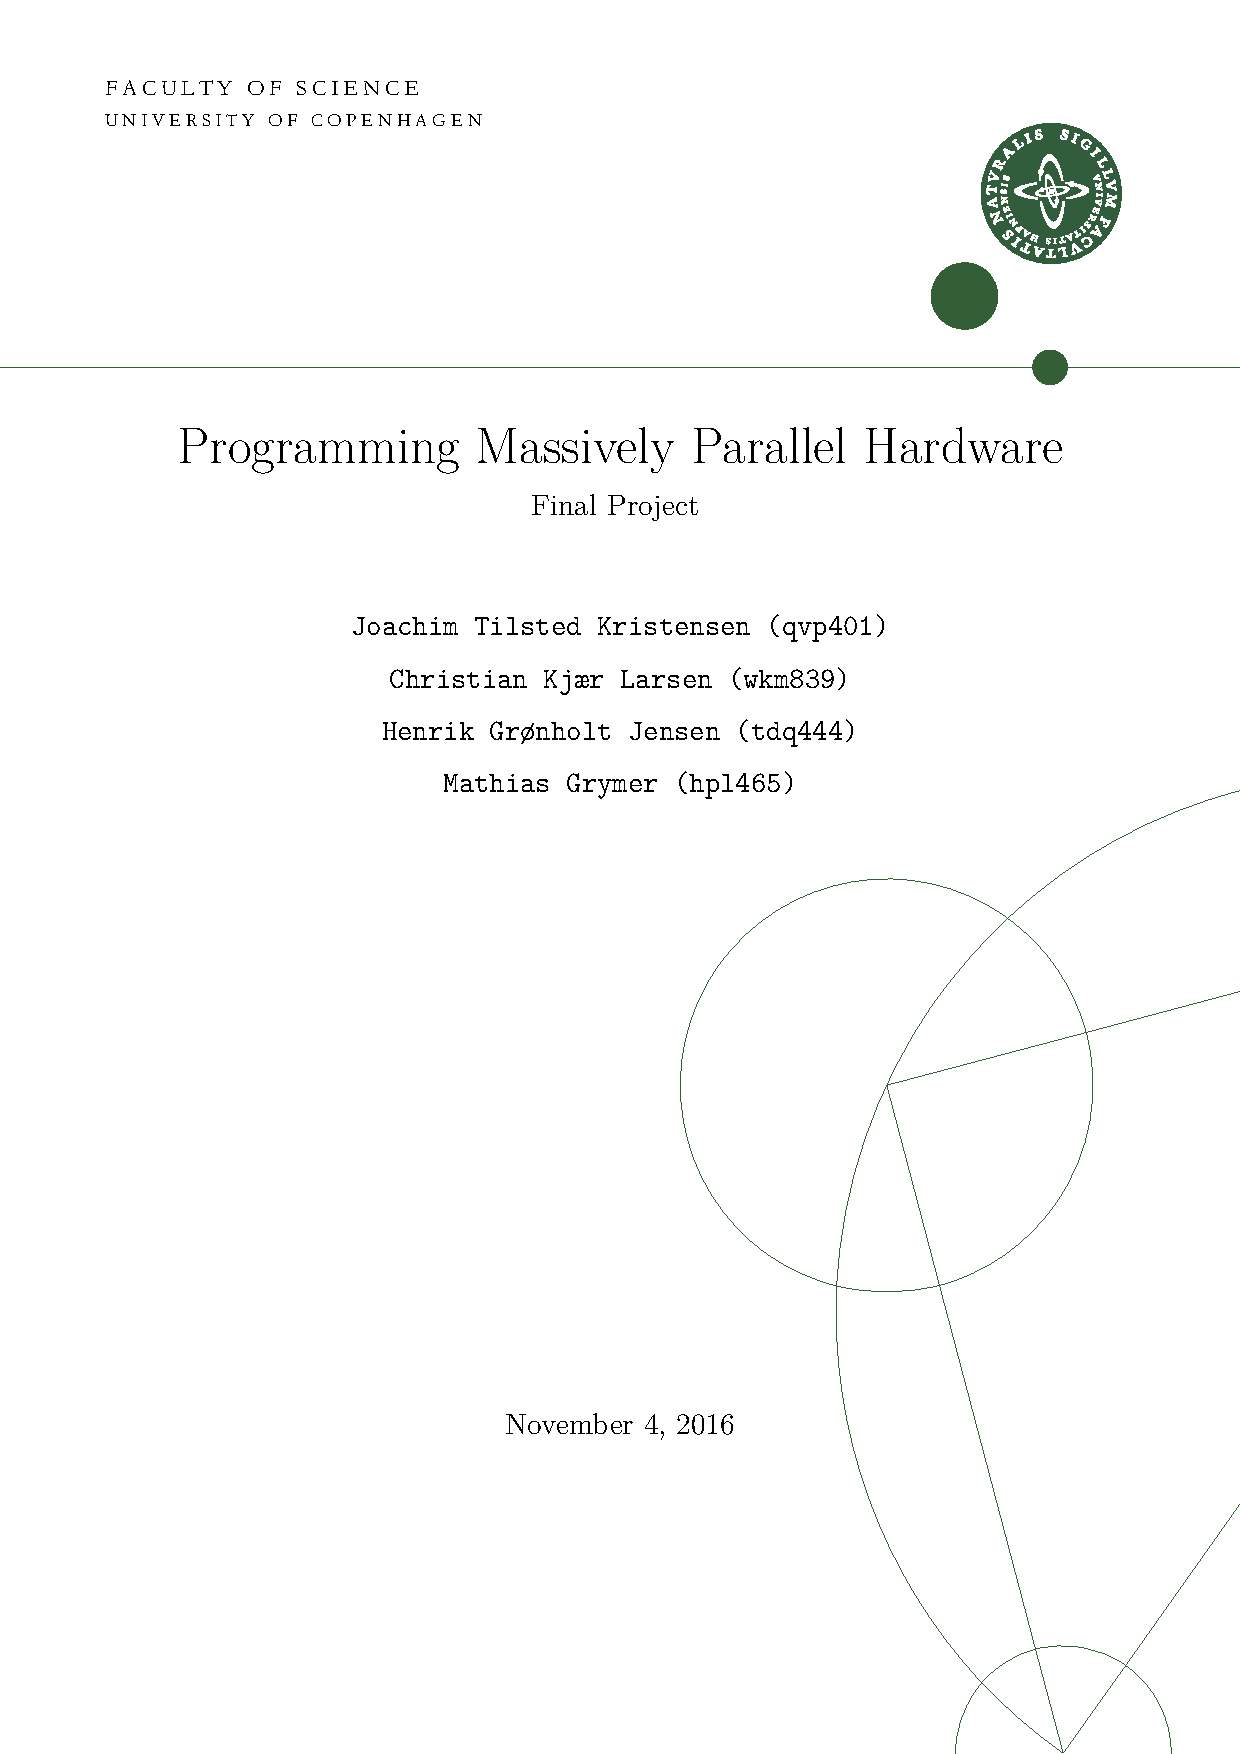
\includepdf[pages=1]{./frontpage/frontpage.pdf}
\tableofcontents
\newpage

\section{Project Introduction}
A histogram is a density estimate over a distribution of data.
It is quintessential to quality control, distribution estimation,
and similarity measures when working with large datasets.
As it is naively parallelizable and scales with the size of the input,
a parallel solution is preferable when the input is large.
However, when it comes to real world unsorted data,
histograms are computationally inefficient due to the random memory access
caused by the counting of how many values fall into each bin.
In this project, we implement a CUDA-based solution for building
a 1D histogram in parallel and benchmark the scalability of our solution with
the CPU and the naive GPU versions.
We also investigate how to efficiently solve the problem when the dataset
is larger than the available (device) memory on the GPU
using streaming techniques.

\section{Design Overview - From CPU to GPU}
Building a histogram in parallel is a straightforward map-reduce problem.
It can be thought of as simplistic kernel density estimation where a function $f$
maps frequencies of data \tt{vals} over bins \tt{inds}
and reduces by counting how many values falls into each bin.
The unoptimised pseudo-code for a 1D histogram
would look something like:

\begin{verbatim}
Forall (i = 0; i < size(data); i++)
    Idx = f(data[i])
    hist[Idx]++ // Must be atomic
\end{verbatim}

For an efficient parallel implementation on the GPU,
the reduce-phase becomes the tricky part.
The unknown order of indices from the map-phase prevents us
from working with the data in a coalesced manner during the reduce-phase.
Our solution to this problem is to partially sort the output indices from the
map-phase into intervals (or segments) that each are guaranteed to fit in the
shared memory of a CUDA block (i.e. no indices fall outside the subset of bins
we can hold in shared memory).
Each block will use its shared memory to create a local histogram
and atomically add this to a global histogram residing on the GPU.
However, to fully utilize hardware parallelism we are likely to have
each CUDA block working on a large subset of data that will
span more than one segment (local histogram).
The subset of data (or indices) a block handles is defined as the workload per thread
(\tt{chunk size}) times the number of threads in a block (\tt{#thread pr block}).
This workload depends on the size of the input data vs.
total number of threads available, and is independent of the sorted segments.
Thus, in each block we need to know when to flush a local histogram to global
memory and start a new segment.
The problem is illustrated in Figure \ref{fig:overview} where e.g.
block-0 spans segment-0 and segment-1.

\fig{overview}{the general idea}

Letting a block handle overlapping segments (i.e. creating more local histograms)
is preferable to a more naïve implementation where a block is spawned
for each segment. This is to keep the algorithm work efficient.
The problem with a more naïve version is that there is no way
to guarantee that all blocks have roughly the same workload.
One could easily have a case where certain segments have significantly
more elements than others, leading to bottlenecks where other blocks will
wait for the overworked blocks to finish.

\section{Overview of Implementation}
\fig{device-dia}{figuretext}

\subsection{Optimised for small histograms}
The first step towards the algorithm described previously is an implementation
for histograms less than the size of the shared memory for each CUDA block.
In our case that is 4096/8192 elements (depending on the configuration).
This is just a way of explicitly managing the cache on the CPU, because the
entire histogram fits in the cache anyway.

\begin{itemize}
\item Reset the shared memory for the block.
\item Write the indices (\tt{f(data[i]}) into the shared memory of the block.
\item Commit the block level histogram to global memory.
\end{itemize}

\subsection{Optimised for large histograms}
This is the version of the previous algorithm with additional bookkeeping
to make sure that the segments are written to the correct location in global memory.

\begin{itemize}
\item
  Map f onto the data array
\item
  Partially sort the resulting indices into a number of equivalence classes (segments)
\item
  Calculate the offset for each segment into
  the partially sorted array of indices.
  This is needed to find the segment for each block.
\item
  Reset the shared memory for each block
\item
  Write the indices into the shared memory of the block modulo the shared memory size
\item
  If we change segment,
  we commit the block level histogram to global memory with a certain
  offset and continue with the next segment in the same manner.
\end{itemize}

A lot of details are left out, but they are very specific to the hardware,
and it is a lot easier just to read the CUDA implementation.
This is especially for details regarding the bookkeeping and calculation
of segment offsets.

\section{}
\section{}


% **************** The End ******************
\end{document}
